\maketitle
\tableofcontents
\newpage

\section{Zielsetzung}
Ziel des Versuches ist es, den Transport von Wärmeenergie entgegen der Richtung des Wärmeflusses
zu untersuchen. Wichtige dabei zu beachtende Größen sind die Güteziffer, der Massendurchsatz und
die mechanische Leistung des Kompressors.
\section{Theorie}
Die Wärmeenergie in einem abgeschlossenen System fließt von der warmen Umgebung in die kalte
Umgebung. Um diesen Wärmefluss umzudrehen, muss mechanische Arbeit erbracht werden. So
eine Maschine wird als Wärmepumpe bezeichnet. Aus dem ersten Hauptsatz der Thermodynamik kommt
\begin{equation}
    \symup{Q_1 = Q_2 + A}
    \label{eqn:3}
\end{equation}
Das Verhältnis zwischen transportierter Wärmemenge und aufgewendeter Arbeit ist definiert
als Güteziffer $\nu$
\begin{equation}
    % müssen noch überlegen, ob wir die \nu kursiv machen oder nicht
    \nu = \symup{\frac{Q_1}{A}}
    \label{eqn:4}
\end{equation}
Dabei ist A die aufgewendetet Arbeit und $\symup Q_1$ die an das wärmere Reservoir abgegebene
Wärmemenge. Es gilt zu beachten, dass dies die Güteziffer für idealisierte Bedingungen darstellt.
Eine weitere idealisierte Annahme kommt aus dem zweiten Hauptsatz der Thermodynamik
\begin{equation}
    \symup{\frac{Q_1}{T_1} - \frac{Q_2}{T_2}} = 0
    \label{eqn:5}
\end{equation}
Da die Wärmepumpe nicht reversibel arbeiten kann, gilt für die reale Beziehung
\begin{equation}
  \symup{\frac{Q_1}{T_1} - \frac{Q_2}{T_2}} > 0
  \label{eqn:6}
\end{equation}
Nun ergibt sich für \eqref{eqn:4} aus \eqref{eqn:5} und \eqref{eqn:6}
\begin{equation}
  \begin{split}
    % müssen noch überlegen, ob wir die \nu kursiv machen oder nicht
    \nu_{\symup{ideal}} = \symup{\frac{T_1}{T_1 - T_2}} \\
    \nu_{\symup{real}} < \symup{\frac{T_1}{T_1 - T_2}}
    \label{eqn:7}
  \end{split}
\end{equation}
Aus den Messwerten der Temperaturen gegen die Zeit gewinnt man die später genutzte Formel
für die Berechnung der realen Güteziffer
\begin{equation}
    \nu = \frac{\symup dQ_1}{\symup dt N} = (m_1c_w + m_kc_k) \frac{\symup dT_1}{\symup dt \, N}
    \label{eqn:8}
\end{equation}
mit $m_1c_w$ als Wärmekapazität des Wassers in Reservoir 1, $m_kc_k$ als Wärmekapazität
der Kupferschlange und des Behälters und N als gemittelte Leistungsaufnahme des Kompressors.
Die nächste zu betrachtende Größe ist der Massendurchsatz $\frac{\symup dm}{\symup dt}$, der
sich über den Differentialquotienten berechnet
\begin{equation}
      \frac{\symup dm}{\symup dt} = (m_2 c_w + m_k c_k) \frac{\symup dT_2}{\symup dt \, L}
      \label{eqn:9}
\end{equation}
mit L als Verdampfungswärme.
Als letztes kommt die Formel für die mechanische Kompressorleistung $\symup N_{mech}$
\begin{equation}
    \symup{N_{mech}} = \frac{1}{\kappa - 1} \left(p_b\sqrt[\kappa]{\frac{p_a}{p_b}} - p_a \right) \frac{1}{\rho}
    \frac{\symup dm}{\symup dt}
    \label{eqn:10}
\end{equation}
mit $\kappa$ als Verhältnis der Molwärmen und $\rho$ als Dichte des Gases.
\section{Durchführung}
\subsection{Versuchsaufbau}
Der Versuchsaufbau, siehe \ref{fig:1}, besteht aus den beiden thermisch isolierten Reservoiren, deren Temperatur über zwei
digitale Termometer abgegriffen werden. Zwei Rührmotoren sorgen für die gleichmäßige Durchmischung des Wassers.
Der Drücke $\symup P_a$ und $\symup P_b$ lassen sich an zwei Manometern ablesen. Ein Kompressor
mit angeschlossenem Motor stellt die benötigte mechanische Arbeit A bereit; die aufgewendete Leistung zeigt
ein Wattmeter an. Somit lassen sich alle zu messenden Größen erfassen.
\begin{figure}
  \centering
  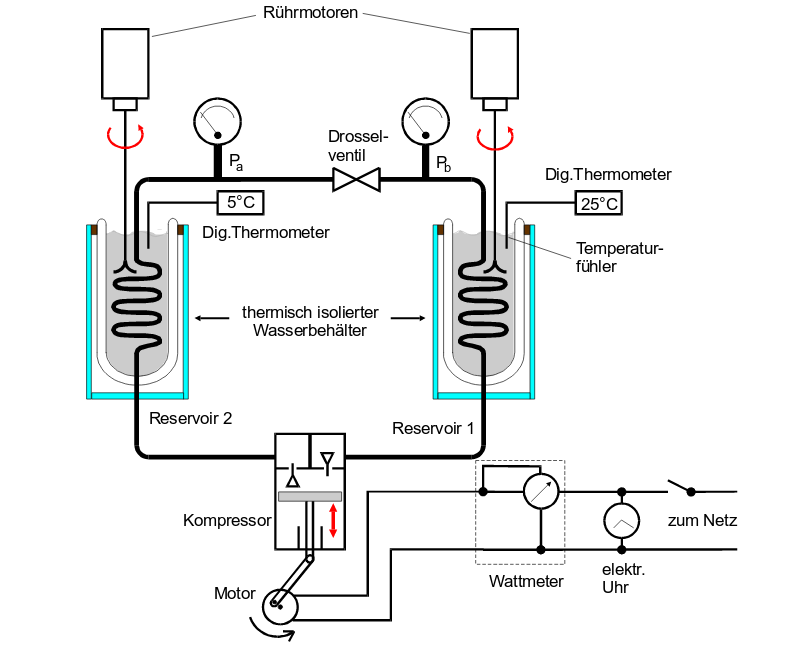
\includegraphics[scale=0.5]{schema.png}
  \caption{Schematische Darstellung des Versuchsaufbaus.}
  \label{fig:1}
\end{figure}
\subsection{Versuchsdurchführung}
Nachdem die Reservoire mit jeweils 3\,$\si{\litre}$ Wasser aufgefüllt wurden,
werden zu Beginn der Messung  die Temperaturen, die Drücke und die Leistung gemessen.
Im $\SI{60}{\second}$ Intervall müssen die oben genannten Größen erfasst werden, bis
$\symup{T_1}$ ungefähr $\SI{50}{\celsius}$ erreicht hat.
\begin{figure}
  \centering
  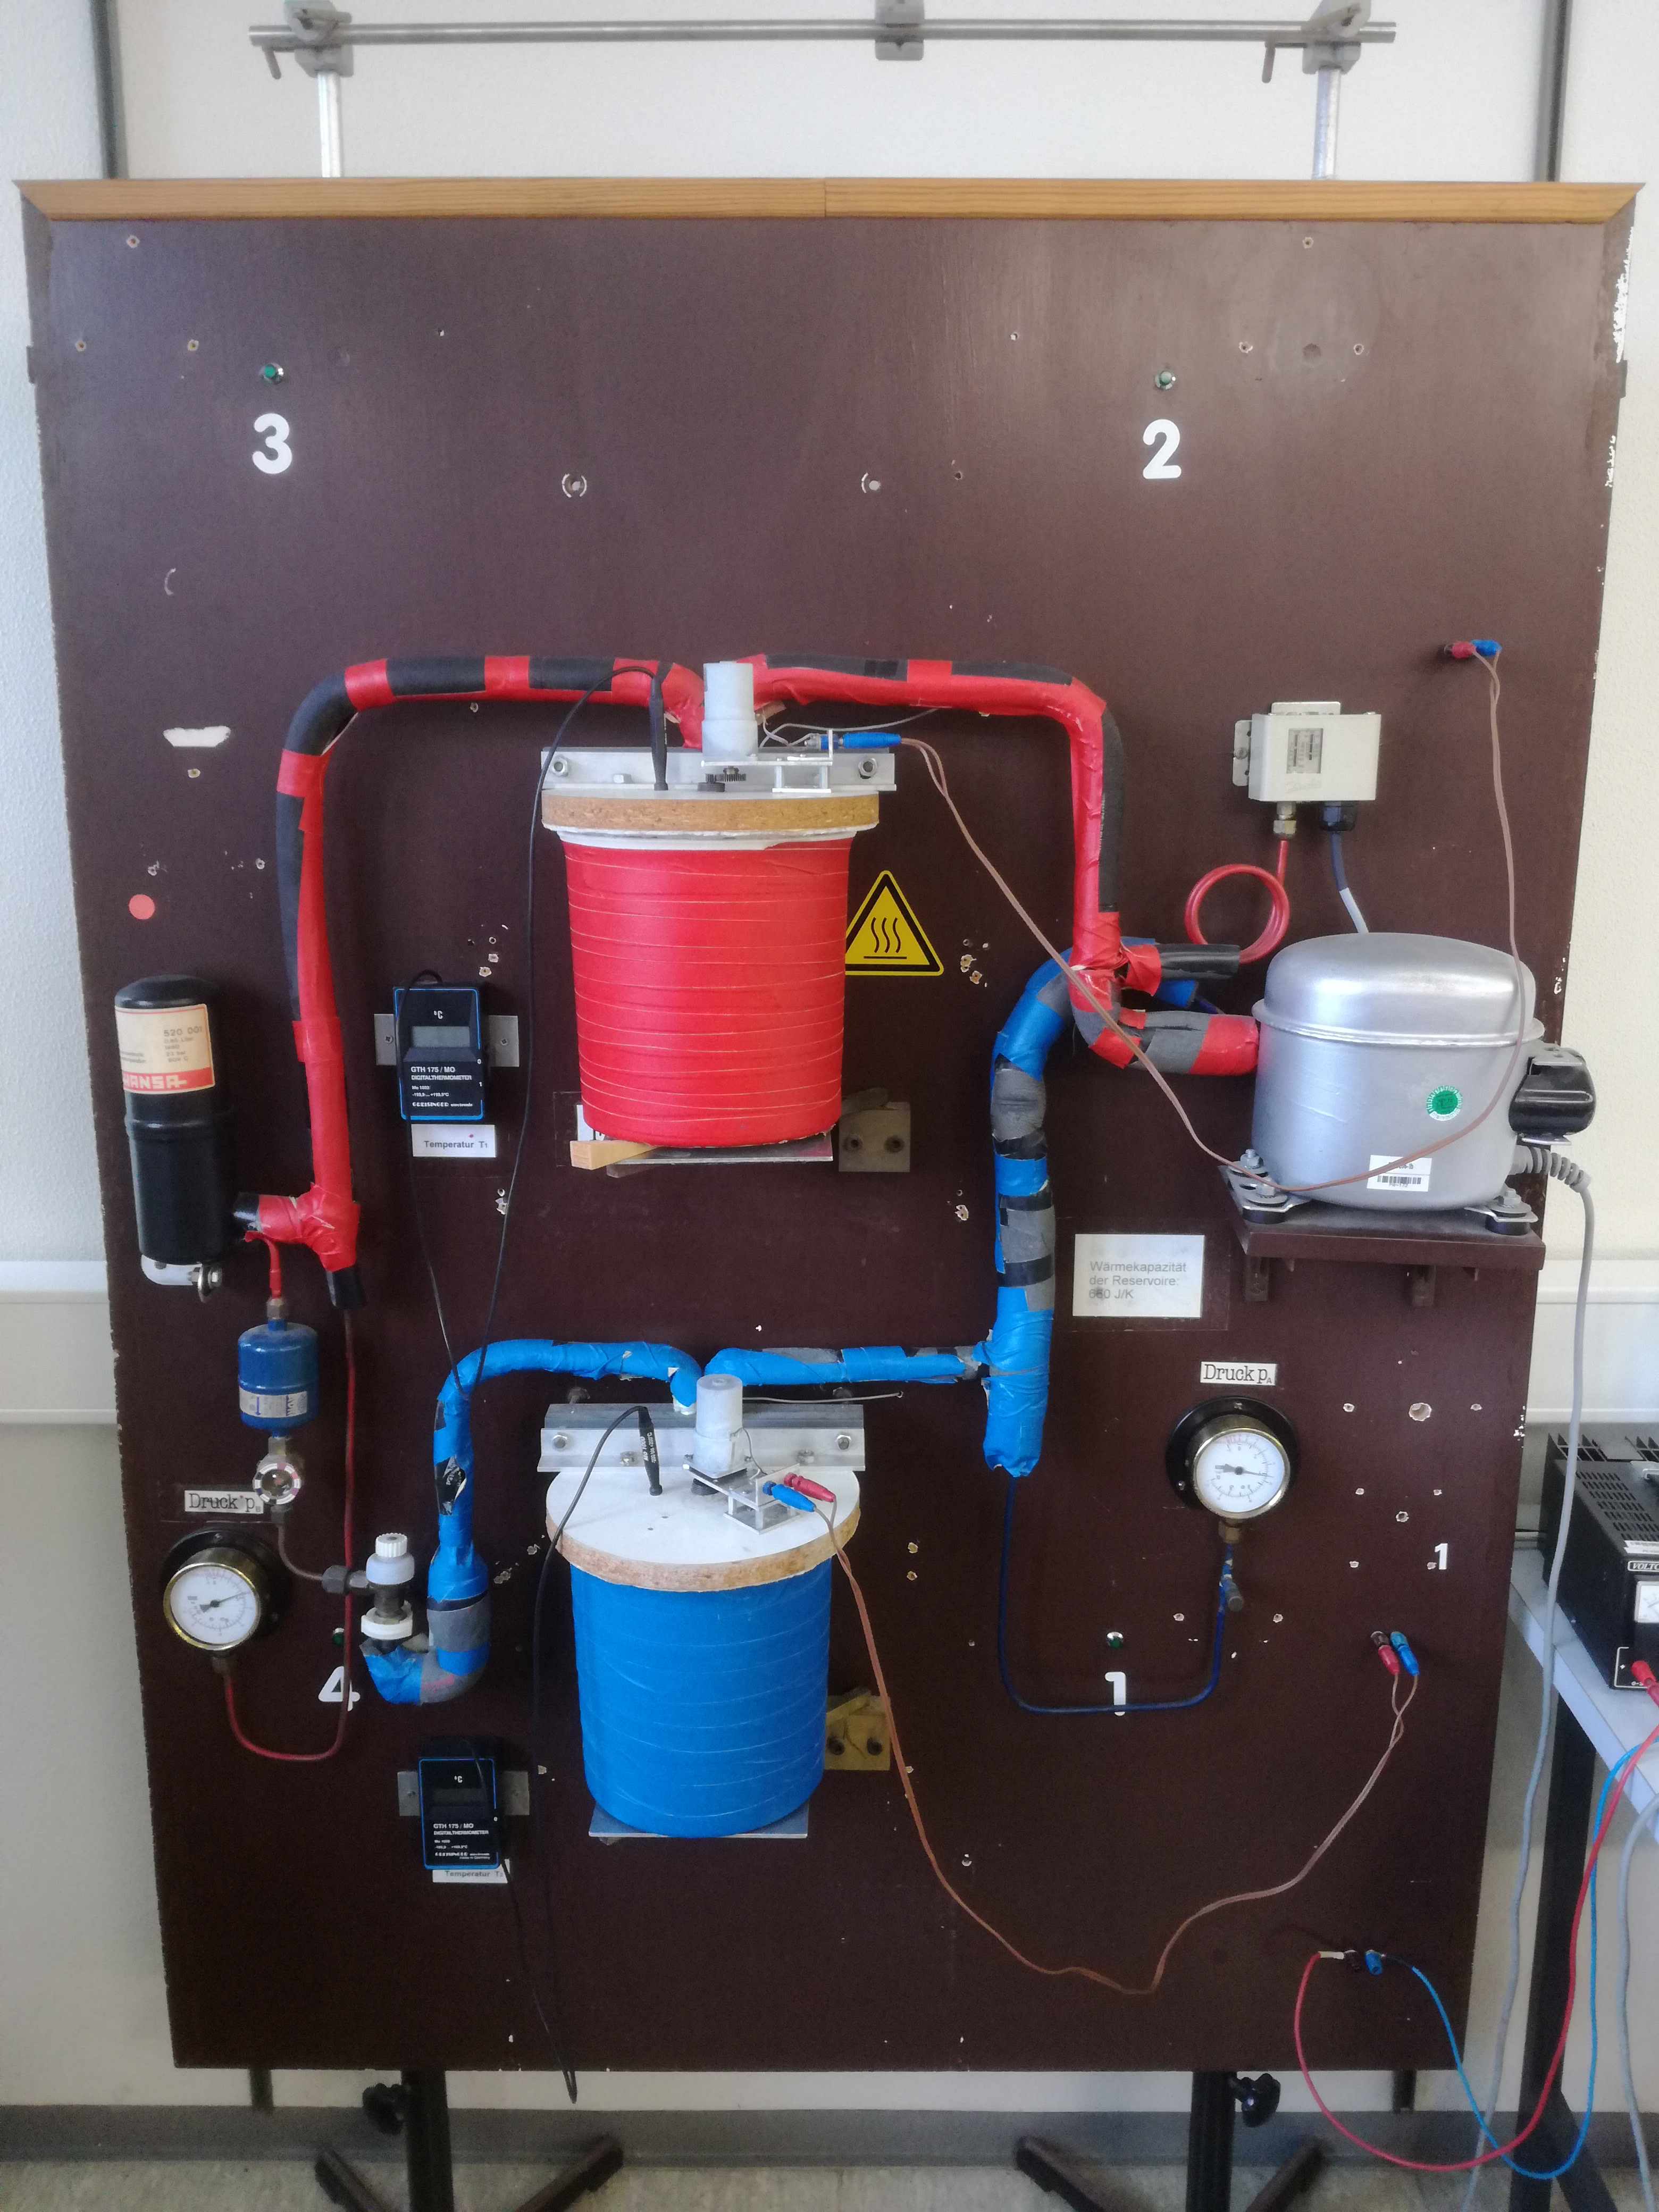
\includegraphics[scale=0.07]{foto.jpg}
  \caption{Der Versuchsaufbau im Foto.}
  \label{fig:2}
\end{figure}
\section{Fehlerrechnung}
Es gibt:
\begin{equation}
  \bar{T} = \frac{1}{n} \sum_{i=1}^{n} T^{i}
  \label{eqn:1}
\end{equation}
den Mittelwert und:
\begin{equation}
  \sigma_{\bar{T}} = \sqrt{\frac{1}{n(n-1)} \sum_{i=1}^{n}(\bar{T}-T_i)^2}
  \label{eqn:2}
\end{equation}
den Fehler des Mittelwertes.
\section{Auswertung}
\section{Diskussion}
\newpage
\nocite{*}
\printbibliography
